\documentclass[a4paper]{article} 
\author{ 
\large
何秦兴 PB16110299 \\[15pt] 
吴雨菲 PB15020525 \\[15pt]
张劲暾 PB16111485 \\[15pt]
}
\title{
	\begin{Huge}
	\textbf
	汽车行业用户观点主题及情感识别\\[26pt]
	\end{Huge}
	{\huge ——数据科学导论期末报告\\[280pt]}
}
\usepackage{xeCJK}
\usepackage{geometry}
\usepackage{ctex}
\usepackage{indentfirst}
\usepackage{listings}
\usepackage[colorlinks,linkcolor=red]{hyperref}
%\usepackage{CJK}
%\setCJKmainfont{AR PL UKai CN}
%\setCJKmainfont{AR PL UMing TW}
\setCJKmainfont{楷体-简 黑体}
\geometry{left=2.5cm,right=2.5cm}
%\setlength{\parindent}{2em}

\begin{document} 
   \maketitle
   \newpage
   \tableofcontents
   \newpage
   \section{题目描述} 
    \subsection{题目背景}
    \paragraph*{
    
 	\begin{large}
    随着政府对新能源汽车的大力扶植以及智能联网汽车兴起都预示着未来几年汽车行业的多元化发展及转变。汽车厂商需要了解自身产品是否能够满足消费者的需求,但传统的调研手段因为样本量小、效率低等缺陷已经无法满足当前快速发展的市场环境。因此,汽车厂商需要一种快速、准确的方式来了解消费者需求。\\[10pt]
   \end{large}
    }
    \subsection{题目任务}
    \paragraph*{
    
 	\begin{large}
    本赛题提供一部分网络中公开的用户对汽车的相关内容文本数据作为训练集,训练集数据已由人工进行分类并进行标记,参赛队伍需要对文本内容中的讨论主题和情感信息来分析评论用户对所讨论主题的偏好。讨论主题可以从文本中匹配,也可能需要根据上下文提炼。\\[10pt]
   \end{large}
    }
    \subsection{数据说明}
    \paragraph*{
    
 	\begin{large}
    训练集数据中主题被分为10类,包括:动力、价格、内饰、配置、安全性、外观、操控、油耗、空间、舒适性。
   \end{large}
    }
    \paragraph*{
    
 	\begin{large}
    情感分为3类,分别用数字0、1、-1表示中立、正向、负向。
   \end{large}
    }
    \paragraph*{
    
 	\begin{large}
    content\_id与content一一对应,但同一条content中可能会包含多个主题,此时出现多条记录标注不同的主题及情感,因此在整个训练集中content\_id存在重复值。\\[10pt]
   \end{large}
    }
    \begin{center}
    \begin{tabular}{|c|c|c|c|}
    \hline 
    字段名称 & 类型 & 描述 & 说明 \\ 
    \hline 
    content\_id & Int & 数据ID & / \\ 
    \hline 
    content & String & 文本内容 & / \\ 
    \hline 
    subject & String & 主题 & 提取或依据上下文归纳出来的主题 \\ 
    \hline 
    sentiment\_value & Int & 情感分析 & 分析出的情感 \\ 
    \hline 
    sentiment\_word & String & 情感词 & 情感词 \\ 
    \hline 
    \end{tabular} 
    \end{center}
    \subsection{评测标准}
    \paragraph*{
    
 	\begin{large}
    本赛题采用F1-Score评价方式。按照“主题+情感分析”识别数量和结果(是否正确)来进行判断,参赛者需要识别文本中可能包含的多个“主题”。匹配识别结果: Tp:判断正确的数量;Fp:判断错误或多判的数量;Fn;漏判的数量.
    \end{large}
    }
    \paragraph*{
    
 	\begin{large}
    当提交的一条数据结果包含“主题+情感值”,如果参赛者对“主题+情感”的判断结果完全正确则计入Tp,如果对“主题”或“情感值”的判断结果错误则计入Fp;如果参赛者未能对某一数据文本判断“主题”或“情感值”给出判断结果,则此条数据不能包含在结果文件中;如果参赛者识别出的“主题+情感值”数量少于测试样本中实际包含的数量,或未对某个测试样本数据给出结果,缺少的数量计入Fn;如果参赛者识别出的“主题+情感值”数量多于测试样本中实际包含的数量,超出的数量计入Fp\\[10pt]
   \end{large}
    }
   \begin{center}
    {\Large \textbf{准确率 : $  P = \frac{T_p}{T_p + F_p} $}}\\[10pt]
    {\Large \textbf{召回率 : $  R = \frac{T_p}{T_p + F_n} $}}\\[10pt]
    {\Large \textbf{F1-Score : $  F1 = \frac{2PR}{P + R} $}}
   \end{center}
   \section{题目分析与方案设计} 
   
  	\subsection{对数据的基本特征分析和设计思路}
  	\paragraph*{
    
 	\begin{large}
    数据基本特征和任务分析:短文本情感分类与主题挖掘,通过将文本映射到向量空间,并将需要预测的情感和主题用独热码表示或编号为类别,将问题转化为学习从文本特征表达到类标签的的映射关系。
    \end{large}
    }
    \paragraph*{
    
 	\begin{large}
    文本的数量特征对模型设计的影响:    
    文本长度普遍较短,可以提取的特征较少,所以需要提取有效的特征;
    多标签问题:每个实例可能对应多个主题标签,而且对于不同的主题标签还有可能是不同的情感分类,这样多主题的数据大概占到总数据的15\%,这一点对于我们采用的主题、情感分开学习,不区分同一ID的不同数据实例的设计方案是不太友好的,参考成功的比赛选手的方案,应该将情感和主题组合\end{large} 
  }得到30个标签进行学习,以解决多标签问题。
    数据数量偏少,只有不到一万条;
    数据质量差,很多主题情感标签模糊,对于很多正面或者负面的评论笼统标注为中性,中性情感标签明显多余另外两类,造成一定的学习过拟合问题,特别是对于LSTM模型的学习影响较大。
   \end{large}
    }
    \subsection{特征提取与模型选择}
    \paragraph*{
    
 	\begin{large}
    对与文本的特征映射,我们采取了两个思路方向,第一是采取将文本分词之后映射到一维的特征向量,比如使用LDA模型或者TFIDF模型,得到特征向量之后交给分类器学习;第二是先训练一个词向量模型,然后将文本映射为一个以词向量为行的特征矩阵,然后卷积池化得到特征向量,交给LSTM模型或者CNN模型学习。
   \end{large}
    }
    \paragraph*{
    
 	\begin{large}
    对于从文本特征空间到标签的映射关系学习,我们将对于情感标签的学习和尝试了逻辑回归模型(LR)、朴素贝叶斯模型(NB)、多层感知机模型(MLP)和多层感知机模型(MLP),最终选择将这些模型进行集成,用最终得到的集成模型分别对情感标签和主题标签进行学习分类。
   \end{large}
    }
   \section{方法说明}
   	\subsection{分词}
   	\paragraph*{
    
 	\begin{large}
    我们首先去除了非中文符号,并且找到了一份通用的汉语停用词表,人工去除了其中可能与主题和情感取向有关的词语,然后分别调用了jieba分词包和THULAC分词包对评论进行分词预处理,jieba分词的结果较为零散,而THULAC的分词结果更加接近于汉语习惯和常用词汇,但在同样的模型测试后,jieba分词得到的效果略好于THULAC,所以我们最终采用了jiaba包做分词处理。
   \end{large}
    }
    \subsection{特征提取}
\subsubsection{隐含狄利克雷主题模型(LDA)}
\paragraph*{

\begin{large}
LDA认为一篇文档的每个词都是通过“以一定概率选择了某个主题,并从这个主题中以一定概率选择某个词语”这样的过程得到。文档到主题服从多项式分布,主题到词服从多项式分布。它采用了词袋模型,将每一篇文档视为一个词频向量。每篇文档代表了一些主题所构成的一个概率分布,而每个主题又代表了一些词所构成的一个概率分布。

\end{large}
}

\paragraph*{
	
	\begin{large}
LDA可使生成的文档中包含多个主题,LDA模型使用下面方法生成一个文档:
	\end{large}	
}

\paragraph*{
	
	\begin{large}
Chooseparameter $\theta \sim p ( \theta )$
	\end{large}	
}

\paragraph*{
	
	\begin{large}
For each of the N words $w_n$
	\end{large}	
}

\paragraph*{
	
	\begin{large}
		Choose a topic $z_n \sim p ( z | \theta )$
	\end{large}	
}

\paragraph*{
	
	\begin{large}
		Choose a word $w_n \sim p ( w | z )$
	\end{large}	
}


\paragraph*{
	
	\begin{large}
		其中N表示要生成的文档的单词的个数,$w_n$表示生成的第n个单词w,$\theta$是一个主题向量,向量的每一列表示每个主题在文档出现的概率,该向量为非负归一化向量;$p(\theta)$是$\theta$的分布,为Dirichlet分布; $z_n$表示选择的主题,$p(z|\theta)$表示给定$\theta$时主题z的概率分布,具体为$\theta$的值,即$p(z=i|\theta)= \theta_i$;$p(w|z)$表示给定z时w的分布,可以看成一个k×V的矩阵,k为主题的个数,V为单词的个数,每行表示这个主题对应的单词的概率分布,即主题z所包含的各个单词的概率,通过这个概率分布按一定概率生成每个单词。
	\end{large}	
}

\paragraph*{
	
	\begin{large}
这种方法首先选定一个主题向量$\theta$,确定每个主题被选择的概率。然后在生成每个单词的时候,从主题分布向量$\theta$中选择一个主题z,按主题z的单词概率分布生成一个单词。
	\end{large}	
}

\paragraph*{
	
	\begin{large}
LDA的联合概率为:
	\end{large}	
}

$p ( \theta , \mathbf { z } , \mathbf { w } | \alpha , \beta ) = p ( \theta | \alpha ) \prod _ { n = 1 } ^ { N } p \left( z _ { n } | \theta \right) p \left( w _ { n } | z _ { n } , \beta \right)$

\paragraph*{
	
	\begin{large}
其图模型如下图:
	\end{large}	
}

\begin{center}
	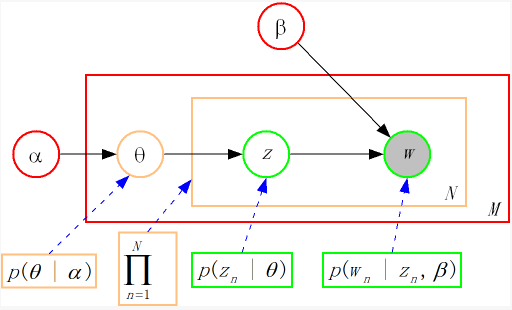
\includegraphics[width=0.8\linewidth]{8.PNG}
\end{center}

\paragraph*{
	
	\begin{large}
从上图可以看出,LDA的三个表示层被三种颜色表示出来:
	\end{large}	
}

\paragraph*{
	
	\begin{large}
(1)corpus-level(红色):$\alpha$和$\beta$表示语料级别的参数,也就是每个文档都相同,因此生成过程只采样一次。
	\end{large}	
}

\paragraph*{
	
	\begin{large}
	(2)document-level(橙色):$\theta$是文档级别的变量,每个文档对应一个$\theta$,也就是每个文档产生各个主题z的概率是不同的,所有生成每个文档采样一次$\theta$。
	\end{large}	
}

\paragraph*{
	
	\begin{large}
		(3)word-level(绿色):z和w都是单词级别变量,z由$\theta$生成,w由z和$\beta$共同生成,一个 单词w对应一个主题z。
	\end{large}	
}

\paragraph*{
	
	\begin{large}
		LDA模型主要是从给定的输入语料中学习训练两个控制参数$\alpha$和$\beta$,学习出了这两个控制参数就确定了模型,便可以用来生成文档。其中$\alpha$和$\beta$分别对应以下各个信息:
	\end{large}	
}


\paragraph*{
	
	\begin{large}
$\alpha$:分布$p(\theta)$需要一个向量参数,即Dirichlet分布的参数,用于生成一个主题$\theta$向量;
	\end{large}	
}


\paragraph*{
	
	\begin{large}
	$\beta$:各个主题对应的单词概率分布矩阵$p(w|z)$。
	\end{large}	
}

\paragraph*{
	
	\begin{large}
把w当做观察变量,$\theta$和z当做隐藏变量,就可以通过EM算法学习出$\alpha$和$\beta$,每次E-step输入$\alpha$和$\beta$,计算似然函数,M-step最大化这个似然函数,算出$\alpha$和$\beta$,不断迭代直到收敛。
	\end{large}	
}



\subsubsection{词袋模型(BOW)}
\paragraph*{

\begin{large}
词袋模型忽略文本的语法和语序,用一组无序的单词来表达一段文本,文本中每个词的出现都是独立的,不依赖于其他词是否出现。首先将文本进行分词,去除停用词,再将每段文本表示为一个数值型向量,形成词袋模型。
\end{large}	
}
\subsubsection{TFIDF}
\paragraph*{

\begin{large}
TFIDF模型用于评估某个词对于一段文本的重要程度。该词的重要性随着它在文本中出现的次数增多而上升,同时会随着它在语料库中出现的频率增多而下降。
\end{large}
}

 	\paragraph*{

\begin{large}
词项t的词项频率tf(t,d)(term frequency)是指词项t在文档d中出现的次数,常采用归一化处理,即词项t在文档d中出现次数count(t, d)和文档d中总词数size(d)的比值:
\end{large}
}

  	\paragraph*{

\begin{large}
tf(t,d) = count(t, d) / size(d) 
\end{large}
}

 	\paragraph*{

\begin{large}
词项t的逆向文档频率idf (inverse document frequency),即文档总数n与出现词项t的文档数目比值的对数:
\end{large}
}

 	\paragraph*{

\begin{large}
idf = log(n / docs(t)) 
\end{large}
}
      	\paragraph*{

\begin{large}
idf是反映词项t信息量的指标,词项信息量越大,idf值越大。
\end{large}
}
  	\paragraph*{

\begin{large}
词项的tfidf权重是tf权重与idf权重的乘积,随着词项频率的增大而增大,随着词项罕见度的增大而增大。
\end{large}
}

  	\paragraph*{

\begin{large}
可用于关键词抽取,将词项按照TFIDF权重排序,排在前几名的为关键词。
\end{large}
}
     \subsubsection{输入LSTM的词向量矩阵}
     % 词向量 部分 begin
 		\paragraph{}
 词向量是NLP中最基本的概念之一,词向量将抽象的语言符号化数学化。主要分为两种:
 \subparagraph{one-hot representation:\\}


    举个例子:\\
    “话筒”表示为 [0 0 0 1 0 0 0 0 0 0 0 0 0 0 0 0 …]\\
    “麦克”表示为 [0 0 0 0 0 0 0 0 1 0 0 0 0 0 0 0 …]\\
    每个词都是茫茫 0 海中的一个 1。 



   \subparagraph{distributed  representation:\\}
    形如[0.792, −0.177, −0.107, 0.109, −0.542, …]
  \paragraph*{
  
  \begin{large}
   Distributed representation 最大的贡献就是让相关或者相似的词,在距离上更接近了。向量的距离可以用最传统的欧氏距离来衡量,也可以用 cos 夹角来衡量。用这种方式表示的向量,“麦克”和“话筒”的距离会远远小于“麦克”和“天气”。可能理想情况下“麦克”和“话筒”的表示应该是完全一样的,但是由于有些人会把英文名“迈克”也写成“麦克”,导致“麦克”一词带上了一些人名的语义,因此不会和“话筒”完全一致。
   \end{large} 
  }
   \paragraph*{
   
   \begin{large} 
   我使用的就是分布式表示,即词嵌入(word embedding),我在实现时直接利用了python gensim包里的word2vec。
   \end{large}
   }
   
   \paragraph*{
   
   \begin{large}
   Word2vec是一组用于生成单词嵌入的相关模型。这些模型是浅层的双层神经网络,经过训练可以重建语言的语言环境。Word2vec将大量文本作为其输入,并产生通常为几百维的向量空间,语料库中的每个唯一单词在空间中被分配相应的向量。单词向量位于向量空间中,使得在语料库中共享共同上下文的单词在空间中彼此非常接近地定位。
   \end{large}
   }
   \paragraph*{
   
   \begin{large}
   这次实验中我们是在数据集上直接训练的Word2vec模型,并没有借助外部数据训练,简单测试表现训练得到的模型对于主题相关词和情感相关词的判断直观上符合逻辑。然后我们将词向量维度设置为100维并测得每条评论的关键词长度最多为80, 于是我们将每条评论中关键字的特征向量依次排列,不足的padding为零,得到一个100*80的矩阵作为LSTM模型的输入(带卷积池化层转换为一维特征向量)。
   \end{large}
   }
% 词向量 部分 end

\subsection{学习方法}
\subsubsection{逻辑回归模型(LR)}
\paragraph*{

\begin{large}
logistic分布函数是一种Sigmoid函数,该曲线呈S型,以点$\left( \mu , \frac { 1 } { 2 } \right)$为中心对称:
\end{large}
}
\paragraph*{

\begin{large}
$F ( x ) = \frac { 1 } { 1 + e ^ { - ( x - \mu ) / \gamma } }$($\mu$为位置参数,$\gamma$为形状参数)
\end{large}
}

\begin{center}
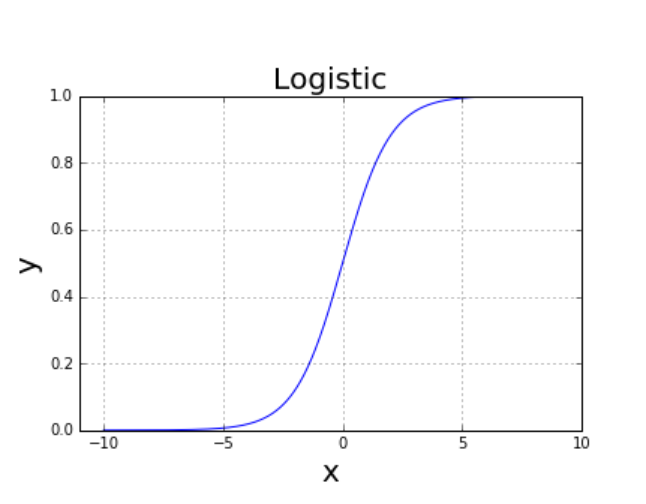
\includegraphics[width=0.8\linewidth]{6.PNG}
\end{center}

\paragraph*{

\begin{large}
利用该函数可将输入转化为一个接近0或1的值,二项logistic回归模型为:
\end{large}
}

$\mathrm { P } ( \mathrm { y } = 1 | \mathrm { x } ) = \frac { e ^ { \omega ^ { T } x + b } } { 1 + e ^ { \mathrm { \omega } ^ { T } x + b } } \)
\( \mathrm { P } ( \mathrm { y } = 0 | \mathrm { x } ) = \frac { 1 } { 1 + e ^ { \omega ^ { T } x + b } }$


\paragraph*{

\begin{large}
用极大似然法估计$\omega$和$b$。
\end{large}
}

\paragraph*{

\begin{large}
将上述模型推广可得多分类模型:多项logistic回归模型
\end{large}
}

$P ( y = k | x ) = \frac { e ^ { \omega _ { k } ^ { T } x + b } } { 1 + \sum _ { k } e ^ { \omega _ { k } ^ { T } x + b } }$



\subsubsection{朴素贝叶斯模型(NB)}
\paragraph*{

\begin{large}
朴素贝叶斯法是基于贝叶斯定理与特征条件独立假设的分类方法。对于给定的训练数据集,首先基于特征条件独立假设学习输入与输出的联合概率分布,然后基于此模型,对于输入,利用贝叶斯定理求出使后验概率最大的输出。
\end{large}
}
\paragraph*{

\begin{large}
由贝叶斯定理(其中, $\omg
_i$是特征词,$c_j$是类别)
\end{large}
}

$P \left( c _ { j } | \omega \right) = \frac { P ( \omega | c _ { j } ) * P \left( c _ { j } \right) } { \sum _ { c _ { j } \in C } P ( \omega | c _ { j } ) * P \left( c _ { j } \right) }$

\paragraph*{

\begin{large}
由条件独立性假设
\end{large}
}

$P \left( c _ { j } | \omega \right) = \frac { P \left( c _ { j } \right) * \prod _ { i } P \left( \omega _ { i } | c _ { j } \right) ^ { \omega _ { t } \left( \omega _ { i } \right) } } { \sum _ { c _ { j } \in C } P \left( c _ { j } \right) * \prod _ { i } P \left( \omega _ { i } | c _ { j } \right) ^ { \omega _ { t } \left( \omega _ { i } \right) } }$


\paragraph*{

\begin{large}
由于对每个$c_j$,分母相同。因此
\end{large}
}

$c = \arg \max _ { c _ { j } \in C } \left\{ P \left( c _ { j } \right) * \prod _ { i } P \left( \omega _ { i } | c _ { j } \right) ^ { \omega _ { t } \left( \omega _ { i } \right) } \right\}$



\paragraph*{

\begin{large}
其中,$P(c_j )$是类别$c_j$的先验概率,$P(\omega│c_j )$是特征词$\omega_i$在类别$c_j$中的条件概率,$\omega_t (\omega_i)$是词$\omega_i$的权值。
\end{large}
}

\paragraph*{

\begin{large}
先验概率$P(c_j )$可用极大似然估计法估计,其中$Doc(c_j)$是属于类别$c_j$的文档数, N为文档总数。
\end{large}
}

$P \left( c _ { j } \right) = \frac { \operatorname { Doc } \left( c _ { j } \right) } { N }$

\paragraph*{

\begin{large}
条件概率$P(\omega_i│c_j )$也可用极大似然估计法估计
\end{large}
}

$P \left( \omega _ { i } | c _ { j } \right) = \frac { \text {weight} \left( \omega _ { i } | c _ { j } \right) } { \sum _ { i } \text { weight } \left( \omega _ { i } | c _ { j } \right) }$

\paragraph*{

\begin{large}
其中,$weight(\omega_i│c_j )$是词$\omega_i$在属于类别$c_j$的文本中的权值之和。
\end{large}
}


\paragraph*{

\begin{large}
但是,如果训练语料中词$\omega_i$在属于类别$c_j$的所有文本中都不出现,则估计的条件概率值为0,这时会影响到后验概率的计算,使分类产生偏差,为解决这个问题,采用贝叶斯估计
\end{large}
}

$P \left( \omega _ { i } | c _ { j } \right) = \frac { \text {weight} \left( \omega _ { i } | c _ { j } \right) + \delta } { \sum _ { i } \text { weight } \left( \omega _ { i } | c _ { j } \right) + \delta * | V | } \)
\( \mathrm { V } = \sum _ { c _ { j } \in C } \sum _ { i } \) weight \( \left( \omega _ { i } | c _ { j } \right)$

\paragraph*{

\begin{large}
其中,$\delta$常取1,称为拉普拉斯平滑,但是,取$\delta=1$增大了训练语料中未出现的特征词的概率,缩小了出现的特征词的概率
\end{large}
}


\subsubsection{多层感知机模型(MLP)}
\paragraph*{

\begin{large}
感知机由两层神经元构成,可对线性可分的数据进行二分类,对于非线性可分的数据,使用多层神经元解决。输入与输出层之间为隐含层。
\end{large}
}

\begin{center}
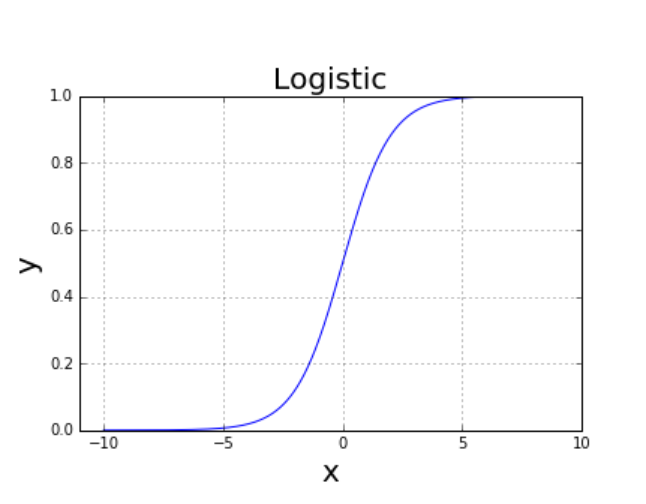
\includegraphics[width=0.8\linewidth]{6.PNG}
\end{center}
   	 
   	 \subsubsection{随机森林模型(RF)}
   	 	% RF 部分 begin
 		\paragraph*{
  
  		\begin{large}
  		对于样本较少的且不太均衡的数据来说,是很容易发生过拟合的。此处使用随机森林的出发点在于对于不平衡的分类资料集来说,随机森林的方法可以平衡误差,且由于随机森林的ensemble特点,它可以产生高准确度的分类器。
		\end{large}}
		\paragraph*{
  
  		\begin{large}
  		随机森林即由很多决策树构成的森林,每棵决策树都是一个分类器(假设现在针对的是分类问题)。
  		\end{large}}
 		\paragraph*{
  
  		\begin{large}
  		随机森林的随机主要体现在两个方面:
  		\end{large}}
 		\paragraph*{
 		
 		\begin{large}
 		\textbf{1. }数据选取的随机,类似于bagging算法中的自助采样法(bootstrap sampling),每一颗决策树都从m个数据中随机有放回地取m个数据,约有近三分之一样本的测试集,三分之二样本的训练集。
 		\end{large}}
 		
 		\paragraph*{
 		
 		\begin{large}
 		\textbf{2. }属性的随机,传统的决策树从当前节点的所有属性中选取一个最优属性,而随机森林的决策树先取一个含k个属性的子集,再在里面取最优,属性的扰动增加了个体学习器的差异度,增强了模型的泛化性能。
 (西瓜书P179,P180)
 		\end{large}}

 		\paragraph*{
 		
 		\begin{large}
 		随机森林算法主要代码(待补充)

 		\lstset{language=python}
 		\begin{lstlisting}
 		\end{lstlisting}
 		\end{large}}
% RF 部分 end

   	 \subsubsection{集成模型(Ensemble)}
   	 % Ensembling 部分 begin
		\paragraph*{
 		
 		\begin{large}
		集成学习通过构建并结合多个学习器来完成学习任务,一般的结构为先产生一组个体学习器,再用某种策略把他们结合起来,典型的有AdaBoost算法、bagging算法和随机森林算法。现在也有人将当下主流的各种NN models进行集成来达到更强的泛化能力与强健性,这与集成学习的概念有所出入但是效果类似。(参考西瓜书P171)
		\end{large}}
\begin{center}
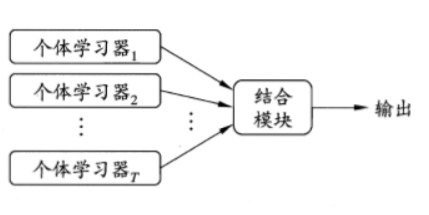
\includegraphics[width=0.8\linewidth]{5.PNG}
\end{center}
\centerline{集成学习示意图}
\subparagraph{Boosting}Boosting是一族可将弱学习器提升为强学习器的算法。这一族算法的工作机制都是类似的:先从初始训练集训练出一个基学习器,再根据基学习器的表现对训练样本分布进行调整,使得先前基学习器做错的训练样本在后续受到更多关注,然后基于调整后的样本分布来训练下一个基学习器
\subparagraph{Bagging}Bagging算法以自助采样法(bootstrap sampling)为基础,从m个数据中\textbf{随机有放回地}取m个数据,约有近三分之一$(\ lim_ {m \to + \infty} \ (1 - \frac{1}{m})^m)$的样本不会被选中,将这些样本作为测试集,其余作为训练集。于是,我们可以采样出T个含m个训练样本的采样集,然后基于每个采样集训练出一个基学习器,再集成,这就是Bagging的基本流程。(参考西瓜书P173,P178)
		\paragraph*{
 		
 		\begin{large}自助法在数据集较小时很有用,并且能从初始数据集中产生多个不同的训练集,这对集成学习有很大的好处。 (西瓜书)
 		在这次实验中我们使用sklearn.ensemble框架中的VotingClassifier集成模型集成了逻辑回归模型(LR)朴素贝叶斯模型(NB)多层感知机模型(MLP)随机森林模型(RF)四种模型对情感和主题进行分类学习。
		\end{large}}

% Ensembling 部分 end
   	 \subsubsection{长短期循环神经网络(LSTM)}
% lstm 部分 begin
%\paragraph{\large 3.3.6 LSTM}.
	\paragraph*{
 		
 		\begin{large}LSTM网络非常适合基于时间序列数据进行分类,处理和预测,因为在时间序列中的重要事件之间可能存在未知持续时间的滞后。LSTM能够捕捉到这些滞后的关联。
 		\end{large}}
\paragraph*{
 		
 		\begin{large}LSTM单元有几种架构。通用架构由存储器单元,输入门,输出门和遗忘门组成。\end{large}}
\subparagraph{一些思考} 有论文对主流的深度学习模型进行了比较,指出LSTM在各类任务中表现优异,有十足的健壮性(robust),唯独在关键词识别(keyphrase recognition)例如情感识别中表现不如其他(当然也不差)。我觉得原因在于句子的情感往往是鲜明的,反应在学习器的输出上的话这些输出值的分布应当不是很均匀的(趋向两级),LSTM捕捉的前后关联自然是没有精准定位情感词来得简单有效。(加上本身中立数据较多,使过拟合更为明显)


\begin{center} %插入的图片居中表示
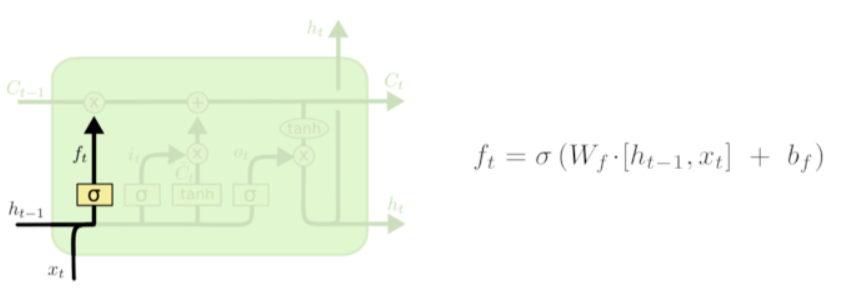
\includegraphics[width=0.8\linewidth]{1.PNG}
\end{center}
\centerline{遗忘门}
\subparagraph{}遗忘门取前一次的细胞状态C$_t$$_-$$_1$为输入,根据需要调权重输出C$_t$$_-$$_1$的一部分

\begin{center}
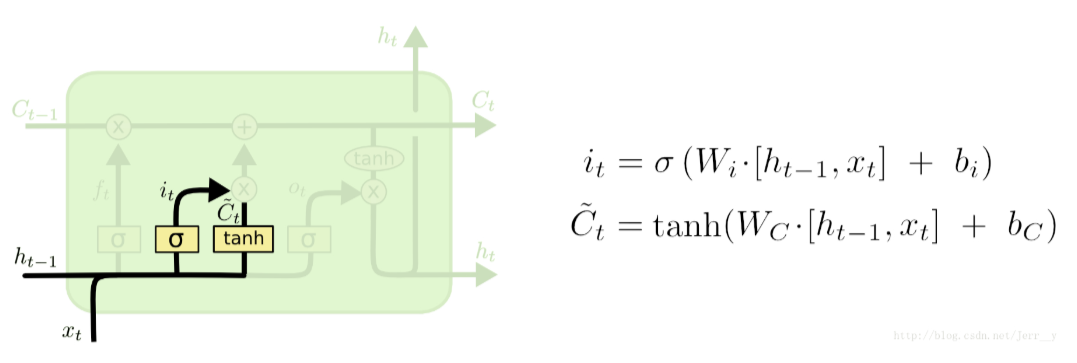
\includegraphics[width=0.8\linewidth]{2.PNG}
\end{center}
\centerline{输入门}
\subparagraph{}输入门决定让多少新的信息加入到细胞的状态中来

\begin{center}
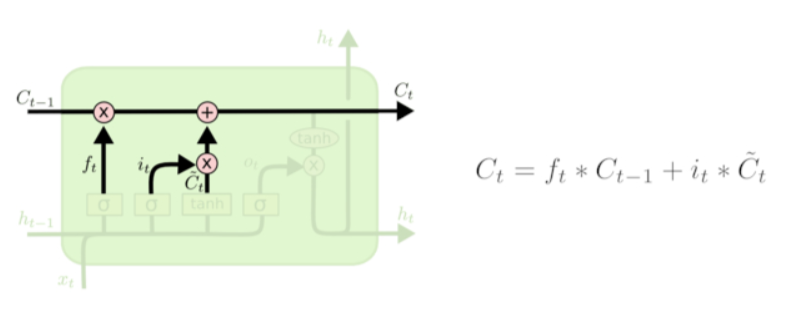
\includegraphics[width=0.8\linewidth]{3.PNG}
\end{center}
\centerline{更新后的细胞状态C$_t$}
\subparagraph{}输入门加上遗忘门就是新的细胞状态C$_t$

\begin{center}
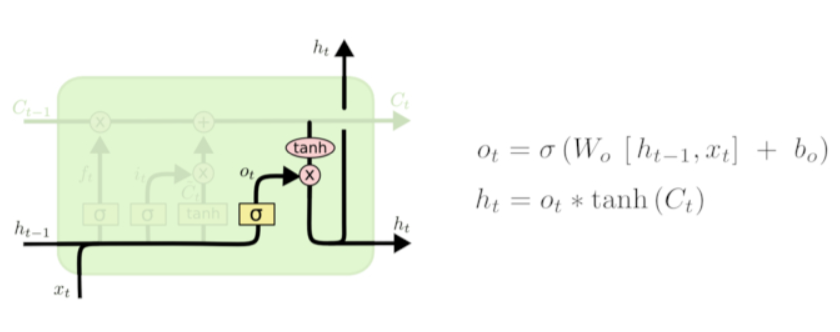
\includegraphics[width=0.8\linewidth]{4.PNG}
\end{center}
\centerline{输出门}
\subparagraph{}最后通过输出门,只输出我们想输出的部分,用于调节整个神经网络信息传递
\newpage
\lstset{language=python}
\begin{lstlisting}[frame=shadowbox]
	model = Sequential()
    model.add(Embedding(output_dim=vocab_dim,
                        input_dim=n_symbols,
                        mask_zero=True,
                        weights=[embedding_weights],
                        input_length=input_length))
    model.add(LSTM(output_dim=50, activation='tanh'))
    model.add(Dropout(0.8))
    model.add(Dense(3, activation='softmax'))
    model.add(Activation('softmax'))

    print('Compiling...')
    model.compile(	loss='categorical_crossentropy',
    				optimizer='adam',
    				metrics=['accuracy'],
    				sample_weight_mode='temporal')

    print("Train...")
    model.fit(	x_train, y_train, 
    			batch_size=batch_size,
                epochs=n_epoch, verbose=1)

    print("Evaluate...")
    score = model.evaluate(x_test, y_test,batch_size=batch_size)
\end{lstlisting}
% lstm 部分 end
    \subsection{提升和改进的思路}
    \paragraph*{
    
    \begin{large}
    首先是对于数据的利用,将给出的情感词利用起来拼在分词结果后面,加强对于情感词的学习,抵消分词不恰当的不利因素,在最终的结果中可以提升一到两个百分点。另外一些没来得及实验的提升设想: 
    1. 对得到的TFIDF向量做PCA主成分分析提升可区分性;
    2. 用引入attention机制的LSTM对情感分类进行学习;
    3. 在词这一层面上对相同情感标签的评论采样生成新的样例,改善类不平衡问题;
    4. 对于主题分类设置阈值,不仅仅是输出最有可能的主题标签,而是将可能性超过阈值的标签分条输出;
    5. 不要将主题和情感分开学习,而是组合得到30种标签去学习,因为数据本来的特征就是对于不同的主题可能有不同的情感态度,这样更接近问题的本质。
    \end{large}
    }
   \section{试验结果}
   	\subsection{线上比赛结果}
   	\noindent
	\large
   最终最佳结果:A榜: 0.60918770000;B榜:0.61174583000\\
   线上其他选手最高成绩:A榜: 0.66085330;B榜:0.66480136

   	\subsection{各种方法的结果与分析}
\noindent
 	\begin{center}
 	\begin{large}
   	\begin{tabular}{|c|c|}
   	\hline 
   	BOW + MLP & 0.46138483000 \\ 
   	\hline 
   	LDA + LR & 0.44940080000 \\ 
   	\hline 
   	LDA + MLP & 0.50000000000 \\
   	\hline 
   	LDA + MLP + LSTM(情感) & 0.41810918000 \\
   	\hline 
   	LDA + RF & 0.53928095000 \\
   	\hline 
   	LDA + RF + LSTM(情感) & 0.44207722000 \\
   	\hline 
   	TFIDF + MLP & 0.56391480000 \\
   	\hline 
   	TFIDF + RF & 0.58521970000 \\
   	\hline 
   	TFIDF + RF + LSTM(情感) & 0.41877496000 \\
   	\hline 
   	TFIDF + ENSMBLE & 0.60918770000 \\
   	\hline 
   	\end{tabular} 
   	\end{large}
 	\end{center}
	我们看到,因为LSTM模型在情感分类上过拟合严重,实际没有什么贡献(也有可能是我们的实现过于粗糙,模型健壮性不好),另外使用LDA特征向量的表现结果比使用TFIDF的效果差很多,可能是LDA模型不适用于这一问题的特征造成的,其余表现情况则是多层感知机模型强于一般的机器学习模型,随机森林模型更强,进一步集成的模型表现出更好的结果。
   	\subsection{没有解决的问题和主要困难}
	\noindent
 	\large
 	1. 因为LSTM模型在对情感分类的学习中表现出严重的过拟合,如何通过采样特征表示得到新的样例 \\
 	2. 对于LDA主题模型实验效果欠佳的解释 \\
 	3. 将标签进行组合之后,每一类标签的实例数量更少,学习效果下降 \\
 	4. 如何学习多主题分类的合理输出阈值 

   \section{附录}
    \subsection{个人收获}
    \noindent
    吴雨菲:\\
    何秦兴:\\
    1. 此次调研的最大收获是对NLP和机器学习有了基本的认识,了解到了不同的模型,也激起了我继续学习相关知识的兴趣。  \\
	2. 感受到了理论和实践之间的巨大Gap,遇到了数据分析过程中一些很实际的问题,真切感受到了数据分析的一些困难,也激起了我对于利用数据科学解决这些困难的兴趣。\\
	3. 理解数据非常重要!恰当得处理数据比模型更重要。\\
	4. 感受到了动手能力的不足,要多锻炼这方面的能力!\\[10pt]
    张劲暾:\\
    1. 学习了关于LDA和LSTM模型的相关知识和相关机器学习框架的编程使用; \\
    2. 参与了一次线上正式比赛,意识到与优秀选手的差距;\\
    3. 积累了团队合作分工、机器学习工程构建的经验。
   	\subsection{分工说明}
   	\noindent
 	吴雨菲:\\
    何秦兴:\\
    1. LSTM模型调研与编程实验\\
    2. 期末报告编写(3.3.4 , 3.3.5, 3.3.6, 3.2.4 部分)\\[10pt]
    张劲暾:(组长)\\
    1. 工作分配协调\\
    2. LDA主题模型调研与编程实验 \\
    3. 框架代码实现与方案具体实现,线上测试提交和比对调整参数 \\
    4. 和何秦兴合作完成LSTM模型编程实现 \\
    5. 期末报告编写(1,2,4 部分)排版 \\
   \section{参考文献}
   \noindent
   1. wikipedia:LSTM\\
   2. 周志华:《机器学习》\\
   3. Wenpeng Yin,Katharina Kann,Mo Yu, Hinrich Schutze.2017.Comparative Study of CNN and RNN for Natural Language Processing  \\
   4. \href {http://www.jmlr.org/papers/volume3/blei03a/blei03a.pdf}
   {Latent Dirichlet Allocation, May 2003, Journal of Machine Learning Research 3(4-5):993-1022, DOI: 10.1162/jmlr.2003.3.4-5.993}\\
   5. \href {http://papers.nips.cc/paper/2698-sharing-clusters-among-related-groups-hierarchical-dirichlet-processes.pdf}
   {Sharing Clusters Among Related Groups:Hierarchical Dirichlet Processes}\\
   6. \href {https://cosx.org/2013/03/lda-math-text-modeling/}
   {LDA-math - 文本建模}\\
   7. \href {http://www.cnblogs.com/pinard/p/6831308.html}
   {文本主题模型之LDA(一) LDA基础}\\
   8. \href {http://www.cnblogs.com/pinard/p/6867828.html}
   {文本主题模型之LDA(二) LDA求解之Gibbs采样算法}\\
   9. \href {http://www.cnblogs.com/pinard/p/6873703.html}
   {文本主题模型之LDA(三) LDA求解之变分推断EM算法}\\
   10. \href {https://blog.csdn.net/pipisorry/article/details/42560693}
   {主题模型TopicModel:Unigram、LSA、PLSA模型}\\
   11. \href {https://blog.csdn.net/pipisorry/article/details/42649657}
   {主题模型TopicModel:隐含狄利克雷分布LDA}\\
   12. \href {https://www.cnblogs.com/jiang1st2010/archive/2013/05/12/3076331.html}
   {Dirichlet Process 和 Hierarchical Dirichlet Process}\\
   13. \href {https://blog.csdn.net/sysuhu/article/details/54378468}
   {分层Dirichlet过程(HDP)的理解}\\
   14. \href {http://www.datalearner.com/blog/1051487944219663}
   {层次狄利克雷过程(Hierarchical Dirichlet Processes)}\\
   15. \href {https://blog.csdn.net/u012845311/article/details/73548882}
   {自然语言处理模型(一):一文读懂TF-IDF} \\
   16. \href {http://www.52nlp.cn/tag/tf-idf}
   {非主流自然语言处理——遗忘算法系列(四):改进TF-IDF权重公式}\\   
   17. 李航 统计学习方法 清华大学出版社\\
   18. \href {https://blog.csdn.net/xholes/article/details/78461164}
   {多层感知机:Multi-Layer Perceptron}\\
   19. \href {http://blog.sina.com.cn/s/blog\_8eee7fb60101czhx.html}
   {LDA(Latent Dirichlet Allocation)主题模型算法}
   
   
   
\end{document}
